\begin{table}[t]
\centering\small
\caption{Test results on the grouped split (9{,}333 test graphs, mostly $L=11,12$). MRE = mean
relative error of $\mathcal{P}$ in \% (mean $\pm$ std over 2 seeds for GNNs); $R^2_{\text{w}}$ = within-loop $R^2$
of $\log\mathcal{P}$. $^\dagger$Uses the Hepp bound, an expensive input, so it is a reference
rather than a competitor. Constant-feature GNNs are trained without BatchNorm.}
\label{tab:main}
\begin{tabular}{lcc}
\toprule
Non-GNN baseline & MRE (\%) & $R^2_{\text{w}}$\\
\midrule
\tabinput{table_base.tex}
\bottomrule
\end{tabular}

\vspace{0.6em}
\setlength{\tabcolsep}{4pt}
\begin{tabular}{l cc cc cc}
\toprule
& \multicolumn{2}{c}{GCN} & \multicolumn{2}{c}{GraphSAGE} & \multicolumn{2}{c}{GIN}\\
\cmidrule(lr){2-3}\cmidrule(lr){4-5}\cmidrule(lr){6-7}
Node features & MRE (\%) & $R^2_{\text{w}}$ & MRE (\%) & $R^2_{\text{w}}$ & MRE (\%) & $R^2_{\text{w}}$\\
\midrule
\tabinput{table_main.tex}
\bottomrule
\end{tabular}
\end{table}

\begin{figure}[t]
\centering
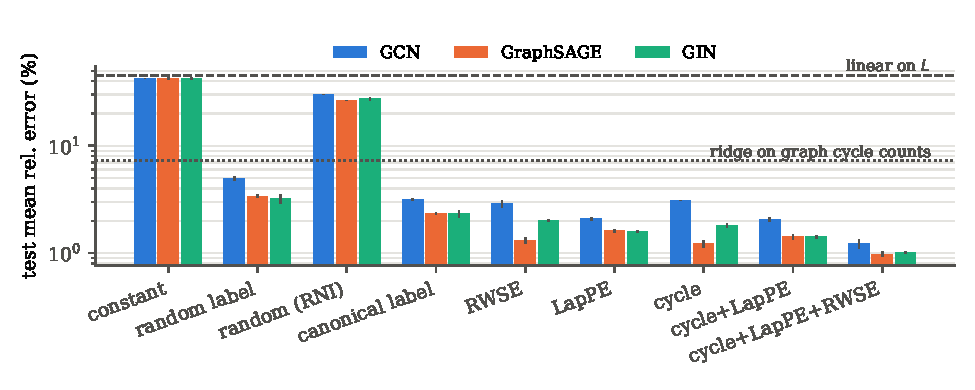
\includegraphics[width=\linewidth]{../figures/ablation.pdf}
\vspace{-1.8em}
\caption{Node-feature ablation (log scale; error bars are $\pm$1 std over 2 seeds). Dashed and
dotted lines show the non-GNN baselines. Constant features cannot beat the linear-in-$L$ baseline
and Gaussian random features barely do; random one-hot labels already help (3--5\%), and every
explicit structural encoding beats ridge regression on the same cycle information by
$2.4$--$7.5\times$.}
\label{fig:ablation}
\end{figure}

\begin{figure}[t]
\centering
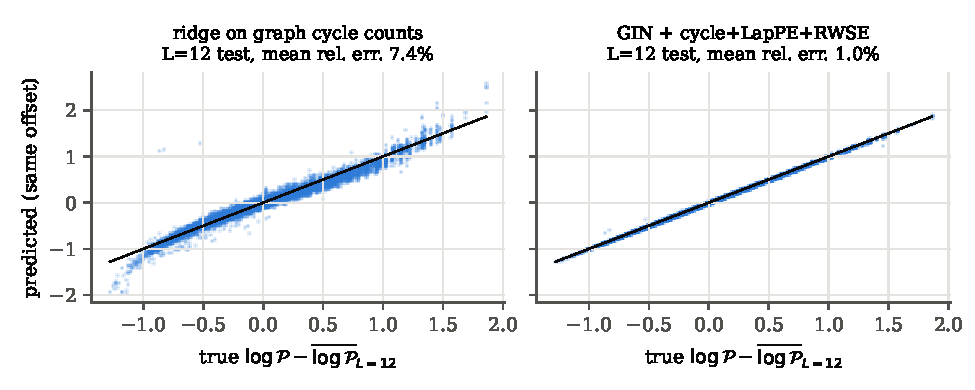
\includegraphics[width=\linewidth]{../figures/scatter_best.pdf}
\vspace{-1.8em}
\caption{Predicted versus true $\log\mathcal{P}$ for the $L=12$ test graphs, after subtracting
the mean $\log\mathcal{P}$ at $L=12$ so that only the hard, within-loop variation is shown. Left:
ridge regression on graph-level cycle counts. Right: the best GNN by validation error.}
\label{fig:scatter}
\end{figure}

Table~\ref{tab:main} and Figure~\ref{fig:ablation} summarize all runs; the main findings follow.

\paragraph{1. Structure-free GNNs cannot beat linear regression, as theory predicts.}
With constant node features all three architectures reach 42.3--42.6\% MRE and a within-loop $R^2$
of $-0.03$. That is the per-loop-mean predictor, exactly as the 1-WL argument of
Section~4 requires: no amount of message passing extracts structure from a regular graph with
featureless nodes. Gaussian random features (RNI) break the symmetry but only reach 26--30\% MRE.
\emph{Random one-hot labels} (a fresh random permutation at every forward pass) do much
better, at 3.0--4.9\%. Our interpretation is that one-hot labels from a small alphabet act as unique node
identifiers: a node can recognize its own label returning after $k$ hops and thus implicitly count
cycles, which continuous Gaussian noise makes much harder to learn. Arbitrary labels are therefore
not hopeless, but they need test-time randomness, are not invariant, and remain about $3\times$ worse than
explicit structural features.

\paragraph{2. Structural node features are what make GNNs work.} Every structural encoding gives
1--3\% MRE and within-loop $R^2>0.994$. The best configuration, cycle participation + LapPE + RWSE,
reaches \textbf{0.97\,$\pm$\,0.05\%} MRE with GraphSAGE and 1.02\% with GIN, which is $47\times$ better than linear
regression on $L$ and $7.5\times$ better than ridge regression on the \emph{same} cycle counts pooled to
graph level (7.3\%). Message passing over per-node cycle participation therefore extracts far
more than the graph-level counts that earlier work used (Fig.~\ref{fig:scatter}). The three
encodings are complementary: each alone gives 1.2--3.1\%, and combining them is best for every
architecture. Training is stable: the seed-to-seed std is at most 0.2 percentage points.

\paragraph{3. The dataset's vertex labels are not arbitrary.} One-hot vertex labels taken directly
from the files reach 2.2--3.2\% MRE, close to the structural features. On inspection this is
expected: the files store graphs in nauty's canonical labelling, so labels plus edges determine
the isomorphism class, and the GNN can exploit the canonical ordering. Such features are not
permutation equivariant and would break for graphs from another source. We therefore treat
random-permutation labels as the true ``arbitrary label'' control, and consider this finding a
caution for any work on this dataset.

\paragraph{4. Architecture matters less than features.} With good features GraphSAGE $\approx$ GIN $>$
GCN. GCN is consistently the weakest, plausibly because its symmetric-normalized aggregation mixes a
node's own features with its neighbors' instead of keeping them separate as GraphSAGE's
concatenation and GIN's $(1+\epsilon)$ term do. GIN's extra theoretical expressivity brings no gain
here, which is consistent with point 1: on regular graphs the bottleneck is the input features, not
the injectivity of the aggregator.

\paragraph{5. Gap to the Hepp bound, and extrapolation in $L$.} The expensive Hepp bound alone gives
0.6\% MRE in a ridge model, so our best cheap GNN is not yet as accurate as a predictor built on this
feature (it is $\sim$1.6$\times$ worse), although it needs only per-node cycle counts and spectra. For
comparison, label noise is negligible (median relative uncertainty of the $L=12$ periods is
$6\times10^{-5}$). Table~\ref{tab:extrap} reports a harder and practically more relevant setting:
training only on $L\le 11$ (about 11k graphs) and predicting all 81{,}305 graphs at $L=12$.
Out of the box, every GNN fails to extrapolate (30--58\% MRE, often worse than linear regression),
while ridge on cycle counts degrades more gracefully (19.7\%). The diagnosis is that the networks
must extrapolate the large, trivial growth of $\log\mathcal{P}$ with $L$ through sum-pooled
embeddings of a graph size they have never seen. A one-line change fixes this: subtracting a linear
fit of $\log\mathcal{P}$ on $L$ and training the GNN on the residual (\texttt{--resid\_L}). With it,
GraphSAGE + cycle+LapPE+RWSE predicts the unseen $L=12$ periods with \textbf{4.3\%} MRE
(within-loop $R^2=0.991$), $4.6\times$ better than ridge regression, using only $\sim$10k training graphs.
This is the most encouraging result for the real use case of predicting high-loop periods from
cheaper low-loop data.

\begin{table}[t]
\centering\small
\caption{Extrapolation in loop order: train/validate on $L\le 11$, test on all 81{,}305 $L=12$
graphs (single seed, 80 epochs). Baselines use $L$ as a numeric feature so that they can extrapolate.}
\label{tab:extrap}
\begin{tabular}{lcc}
\toprule
Model & MRE (\%) & $R^2_{\text{w}}$\\
\midrule
\tabinput{table_extrap.tex}
\bottomrule
\end{tabular}
\end{table}

\paragraph{What did not work / lessons.} (i) With BatchNorm, constant-feature models diverged at
evaluation time (MRE $\to\infty$). The cause is degenerate batch statistics, and we re-ran these
controls without normalization. (ii) Our first attempt stored the label feature under a name
containing \texttt{index}, which PyG silently treats as an index tensor and offsets during batching.
(iii) Hyper-parameters (width 64, depth 4, 40 epochs) are untuned. Validation error is noisy at
the initial learning rate and drops as the cosine schedule anneals, and for every run the best
checkpoint lies within the last five epochs (Fig.~\ref{fig:curves}), so longer training will likely
improve all GNN numbers.

\begin{figure}[h]
\centering
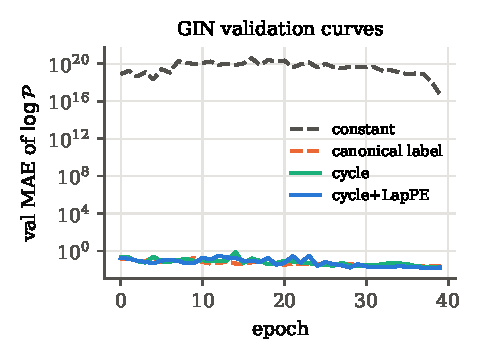
\includegraphics[width=0.85\linewidth]{../figures/curves_gin.pdf}
\vspace{-0.8em}
\caption{Validation MAE of $\log\mathcal{P}$ during training (GIN, seed 0). Curves are noisy at
the initial learning rate and settle as the cosine schedule anneals; the constant-feature
control stays flat at the per-loop-mean level throughout.}
\label{fig:curves}
\end{figure}
